	
		\paragraph{} This section shows how the processes run and interact in the system. 
		We will present processes, that covers most features of our system: Sign in and Car Employment, which includes: Reservation of a car in specific zone, Picking up a reserved car, Riding a car. Employment of a car can be divided into several processes, but we decided to show them in one sequence diagram due to their close interaction.    

	\subsubsection{Sign in}	
		\begin{figure}[h]
			\includegraphics[scale=0.7]{img/SignInSD.png}
		\end{figure}
		
		\paragraph{} This sequence diagram represents the User login. 
		The Guest has to fill the form on the Login page with his credential information and press Login as he's finished. 
		Then the Access Manager is notified that the Guest filled the form and wishes to log in, Access Manager sends this request to System Model to check the data from the form and find it in the database. When the System Model finishes the control of the data, there is to alternative scenarios of what will happen. 
		If the Guest has entered wrong data the Login form, the System Model will send back to Access Manager a message, notifying that the given information was not found in the database, the error message will be displayed on the Login page. 
		If the Guest filled the form with right credentials, then the System Model will confirm the Access Manager the correctness of the information, and the success message will be displayed on the Login Page, after which the Guest will redirected to Main Page as User.           
			
	\newpage
	\subsubsection{Car Employment}	
	
		\begin{figure}[h]
			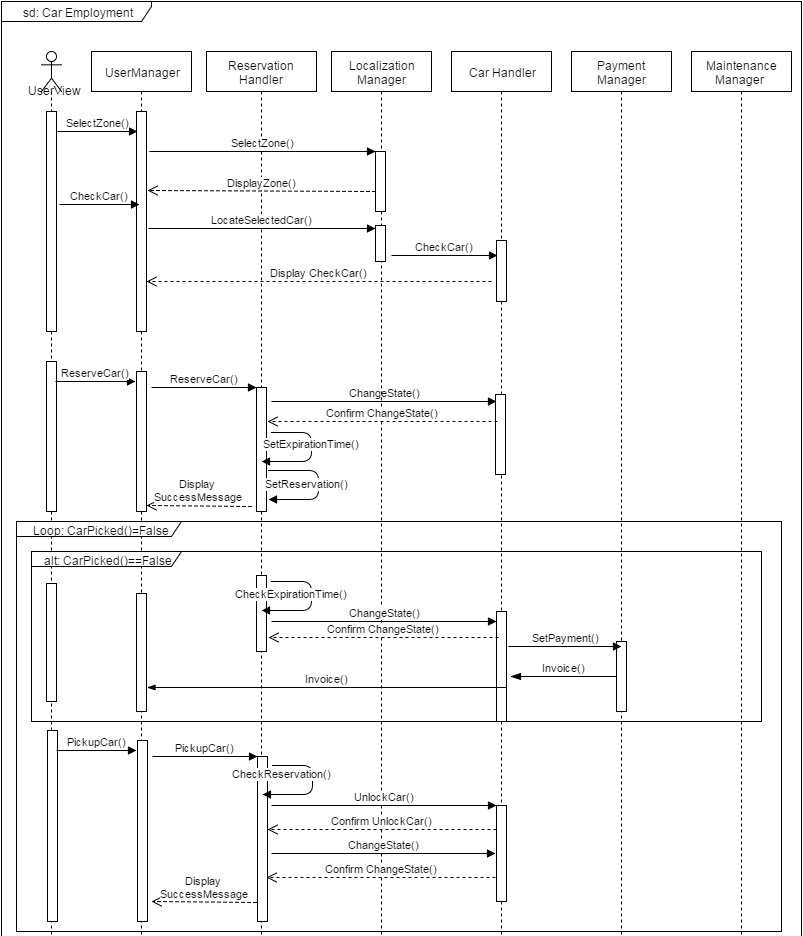
\includegraphics[scale=0.55]{img/CarEmploymentSD1.png}
		\end{figure}
		\newpage
		\begin{figure}[h]
			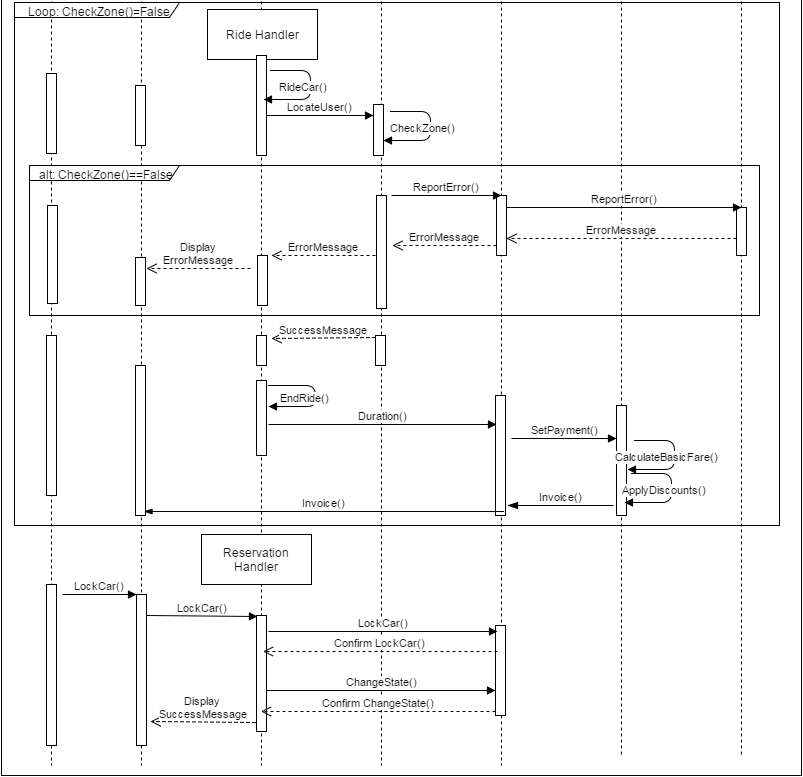
\includegraphics[scale=0.55]{img/CarEmploymentSD2.png}
		\end{figure}
		
		\paragraph{} This sequence diagram shows the employment of car by User.
		User selects the zone on the Main page in order to the system to understand the User's location, this information is sent to Localization Manager, which will save the selected zone, that will be displayed on the Main page. Now User can pick a car only from one specific zone. User selects a car on a Main Page, the request is sent to Localization Manager, that gives detailed location of the car and sends request to check the car to Car Handler, which replies directly to the Main page, where the detailed information about the car is displayed. The User choses to reserve this car, the request is sent Reservation Handler that passes the request to Car Handler to change the state of the car to unavailable. Car Handler answers back and confirms the change of car's state. The Reservation Handler sets the expiration time and registers the reservation, this will display as a message on the Main Page. 
		
		After this procedure User has choice to pick up the reserved car or not.
		
		If by the expiration time the User will not pick up the car, the  Reservation Handler will send the request to Car Handler to change the state of the car back to available, after the Car Handler gives confirmation of change of the state, it also notifies the Payment manager to set the payment (fee), Payment Manager gives back the information about the payment to Car Handler, that will send this information to Main Page, where it will be displayed as a message. User make the payment, the request is sent from Main Page to Car Handler that passes it to Payment Manager, which replies back with the confirmation of  the payment, this information will be displayed on the Main Page as a success message.   
		
		If the User picks up the reserved car on time, the request to pick up the car is sent to Reservation Handler, that checks the correctness of the reservation and sends the request to Car Handler to unlock the car and then to change the state of the cat to in use, Car Handler confirms back both operations, this information is displayed on the Main Page as success message.
		
		While the user rides the car, Ride Handler always keep in track with the location by sending the request to Localization Manager, that Check if the location is still in selected zone. 
		
		If the User left the selected zone, Localization Manager reports the error to Car Handler, that passes it to Maintenance Manager, which replies back the error message, that goes to Localization Manager, Ride Handler and is displayed on the Main Page.
		
		If the User is in the selected zone, then Localization Manager answers the Ride Handler with a success message.  
		
		The User ends the ride, this requests passes from Main Page to Ride Handler, that sends request to Car Handler in order to check the car,   it confirms back with the information about the car. Car Handler sends the Payment Manager request to set the payment. Payment Manager applies the discounts (if there are any) to the payment and answers back to Car Handler, the payment information passes directly to the Main Page. 
		
		User makes payment, this requests is sent from Main Page directly to Car Handler, that passes it to Payment Manager. Payment Manager confirms payment to Car Handler, that sends this information to Main Page that displays it as success message.
		
		User Lock the car, this request is sent from Main Page to Reservation Handler, that sends it to Car Handler and the car answers back with an confirmation. Reservation Handler sends request to Car Handler to change the state of the car to available, Car Handler answers back with confirmation that the state is changed, this information is displayed on the Main Page as success message.    
